%%%%%%%%%%%%%%%%%%%%%%%%%%%%%%%%%%%%%%%%%
% Beamer Presentation
% LaTeX Template
% Version 1.0 (10/11/12)
%
% This template has been downloaded from:
% http://www.LaTeXTemplates.com
%
% License:
% CC BY-NC-SA 3.0 (http://creativecommons.org/licenses/by-nc-sa/3.0/)
%
%%%%%%%%%%%%%%%%%%%%%%%%%%%%%%%%%%%%%%%%%

%----------------------------------------------------------------------------------------
%	PACKAGES AND THEMES
%----------------------------------------------------------------------------------------

\documentclass[xetex,serif,mathserif,14pt]{beamer}

\mode<presentation> {

% The Beamer class comes with a number of default slide themes
% which change the colors and layouts of slides. Below this is a list
% of all the themes, uncomment each in turn to see what they look like.

%\usetheme{default}
%\usetheme{AnnArbor}
%\usetheme{Antibes}
%\usetheme{Bergen}
%\usetheme{Berkeley}
%\usetheme{Berlin}
%\usetheme{Boadilla}
%\usetheme{CambridgeUS}
%\usetheme{Copenhagen}
%\usetheme{Darmstadt}
%\usetheme{Dresden}
%\usetheme{Frankfurt}
%\usetheme{Goettingen}
%\usetheme[hideothersubsections]{Hannover}
%\usetheme{Ilmenau}
%\usetheme{JuanLesPins}
%\usetheme{Luebeck}
%\usetheme{Madrid}
%\usetheme{Malmoe}
%\usetheme{Marburg}
%\usetheme{Montpellier}
%\usetheme{PaloAlto}
%\usetheme{Pittsburgh}
%\usetheme{Rochester}
%\usetheme{Singapore}
%\usetheme{Szeged}
\usetheme{Warsaw}

% As well as themes, the Beamer class has a number of color themes
% for any slide theme. Uncomment each of these in turn to see how it
% changes the colors of your current slide theme.

%\usecolortheme{albatross}
%\usecolortheme{beaver}
%\usecolortheme{beetle}
%\usecolortheme{crane}
%\usecolortheme{dolphin}
%\usecolortheme{dove}
%\usecolortheme{fly}
%\usecolortheme{lily}
%\usecolortheme{orchid}
%\usecolortheme{rose}
%\usecolortheme{seagull}
%\usecolortheme{seahorse}
%\usecolortheme{whale}
%\usecolortheme{wolverine}
\usecolortheme[named=violet]{structure}

%\setbeamertemplate{footline} % To remove the footer line in all slides uncomment this line
%\setbeamertemplate{footline}[page number] % To replace the footer line in all slides with a simple slide count uncomment this line

%\setbeamercolor{frametitle}{fg=red,bg=red!20} % Redefine color of frame title box
%\setbeamercolor*{title}{bg=red,fg=white} % Redefine color of presentation title box
%\setbeamercolor{block title}{fg=black,bg=black!20} % Redefine color of block title %bg=background, fg=foreground
%\setbeamercolor{block body}{fg=black,bg=red!15} % Redefine color of block body

\makeatletter
\setbeamertemplate{footline} % Redefine footer (mainly width of boxes)
{
  \leavevmode%
  \hbox{%
  \begin{beamercolorbox}[wd=.41\paperwidth,ht=2.25ex,dp=1ex,center]{author in head/foot}%
    \usebeamerfont{author in head/foot}\insertshortauthor~~(\insertshortinstitute)
  \end{beamercolorbox}%
  \begin{beamercolorbox}[wd=.34\paperwidth,ht=2.25ex,dp=1ex,center]{title in head/foot}%
    \usebeamerfont{title in head/foot}\insertshorttitle
  \end{beamercolorbox}%
  \begin{beamercolorbox}[wd=.25\paperwidth,ht=2.25ex,dp=1ex,right]{date in head/foot}%
    \usebeamerfont{date in head/foot}\insertshortdate{}\hspace*{2em}
    \insertframenumber{} / \inserttotalframenumber\hspace*{2ex}
  \end{beamercolorbox}}%
  \vskip0pt%
}
\makeatother

%\setbeamertemplate{navigation symbols}{} % To remove the navigation symbols from the bottom of all slides uncomment this line
}

\usepackage{polyglossia} % χρησιμοποιείται για καλύτερη υποστήριξη των Ελληνικών
\usepackage{graphicx} % Allows including images
\usepackage{booktabs} % Allows the use of \toprule, \midrule and \bottomrule in tables
\usepackage{pgfplots} % For drawing the queries
\usepgfplotslibrary{groupplots}
\usetikzlibrary{pgfplots.groupplots}
\usepackage{xcolor} % For colors
\usepackage{tikz}
\usepackage{unicode-math}
\usepackage[framed,numbered,useliterate]{mcode}
\usepackage{textpos}
\pgfplotsset{compat=1.10}

\setmainlanguage[numerals=arabic]{greek} % κύρια γλώσσα
\setotherlanguages{english} % δευτερεύουσα γλώσσα

%----------------------------------------------------------------------------------------
%	TITLE PAGE
%----------------------------------------------------------------------------------------

\title[Κατηγοριοποίηση Κρίνων]{Κατηγοριοποίηση Κρίνων με Χρήση Νευροασαφούς Μοντέλου} % The short title appears at the bottom of every slide, the full title is only on the title page

\author[Χατσατριάν, Κοσματόπουλος]{Άνι Χατσατριάν, Μιχάλης Κοσματόπουλος} % Your name
\institute[ΑΤΕΙΘ] % Your institution as it will appear on the bottom of every slide, may be shorthand to save space
{
Αλεξάνδρειο Τεχνολογικό Εκπαιδευτικό Ίδρυμα Θεσσαλονίκης \\ % Your institution for the title page
\medskip
\textit{\{achatsat, mkosm\}@it.teithe.gr} % Your email address
}
\titlegraphic{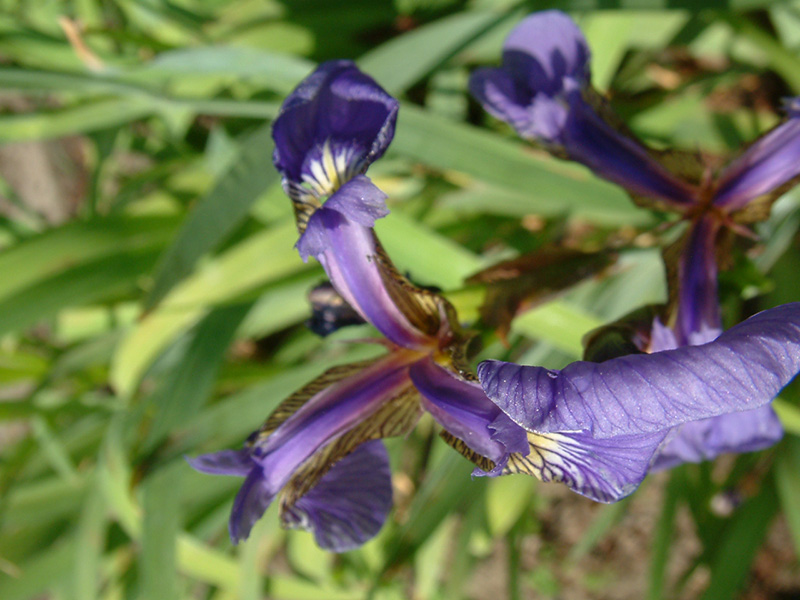
\includegraphics[height=2cm]{images/irisSetosa.jpg} 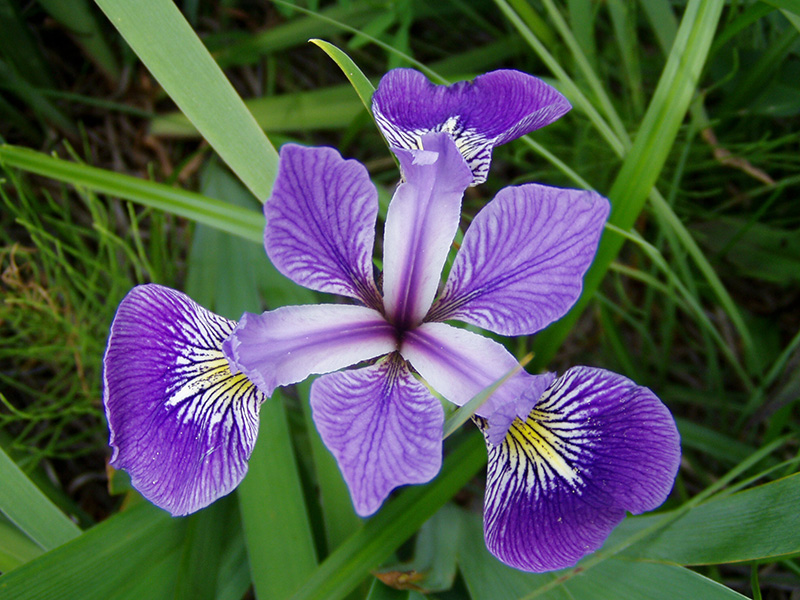
\includegraphics[height=2cm]{images/irisVersicolor.jpg} 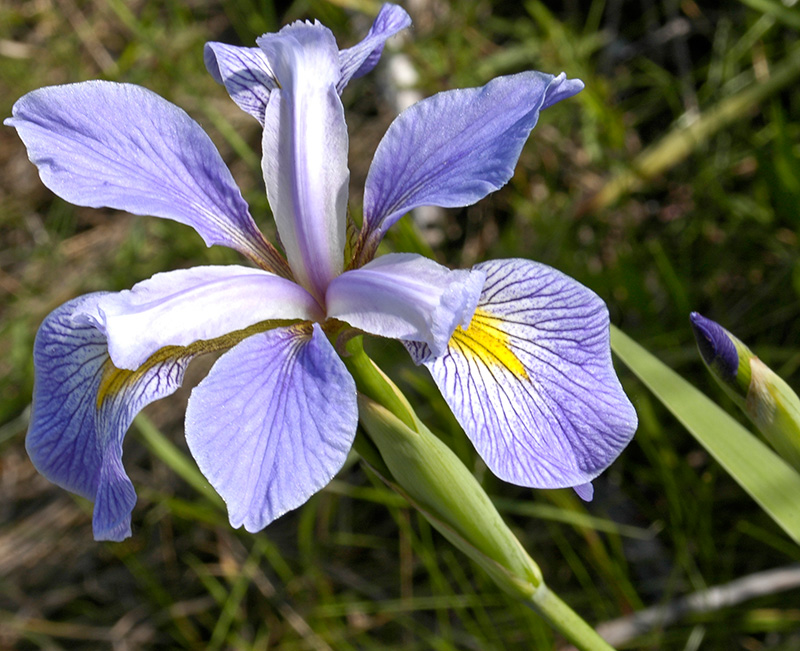
\includegraphics[height=2cm]{images/irisVirginica.jpg}}
\date{23 Μαΐου 2014} % Date, can be changed to a custom date
%\logo{
\includegraphics[height=0.8cm]{images/itLogoWhiteBg.pdf}}
\newfontfamily\greekfont[Script=Greek]{Linux Libertine G} % work-around για bug του polyglossia
\setmainfont[Kerning=On,Mapping=tex-text]{Linux Libertine G} % roman font
%\setmathfont{Latin Modern Math}

\renewcommand{\arraystretch}{1.3} % μεγαλύτερο διάστημα ανάμεσα στις γραμμές πινάκων

\pgfmathdeclarefunction{trig}{1}{%
    \pgfmathparse{%
        (and(   1,    #1<=1)*(0)            +%
        (and(1<#1,    #1<=2)*((#1-1)/(2-1)) +%
        (and(2<#1,     #1<3)*((3-#1)/(3-2)) +%
        (and(1,       #1>=3)*(0)%
    }%
}

\newcommand{\trigLabel}{
    $\mu_A(x) = \left\{
        \begin{array}{lr}
            0 & x \leq a\\
            \frac{x-a}{m-a} & a < x \leq m\\
            \frac{b-x}{b-m} & m < x < b\\
            0 & x \geq b
        \end{array}
    \right.$
}

\newcommand{\trigPlot}{
    \raisebox{-.5\height}{
        \begin{tikzpicture}
            \begin{axis}[
            scale = 0.2,
            axis y line=middle,
            axis x line=bottom,
            xtick={1,2,3},
            xticklabels={$a$, $m$, $b$},
            xticklabel style={anchor=base, yshift=-6pt},
            ymin=0,
            ymax=1.1,
            ytick={0.00001, 1},
            yticklabels={$0$, $1$},
            major y tick style = transparent]
                \addplot[domain=0:4, blue, samples=100, ultra thick] {(trig(x))};
            \end{axis}
        \end{tikzpicture}
    }
}

% ---------------------------

\pgfmathdeclarefunction{trapezoid}{5}{
    \pgfmathparse{%
        (and(     1,   #1<#2)*(0)           +%
        (and(#2<=#1,  #1<=#3)*((#1-#2)/(#3-#2)) +%
        (and(#3<=#1,  #1<=#4)*(1) +%
        (and(#4<=#1,  #1<=#5)*((#5-#1)/(#5-#4)) +%
        (and(1,        #1>#5)*(0)%
    }%
}

\newcommand{\trapLabel}{
    $\mu_A(x) = \left\{
        \begin{array}{lr}
            0 & x < a\\
            \frac{x-a}{b-a} & a \leq x \leq b\\
            1 & b \leq x \leq c\\
            \frac{d-x}{d-c} & c \leq x \leq d\\
            0 & x > d
        \end{array}
    \right.$
}

\newcommand{\trapPlot}{
    \raisebox{-.5\height}{
        \begin{tikzpicture}
            \begin{axis}[
            scale = 0.2,
            axis y line=middle,
            axis x line=bottom,
            xtick={1,2,3,4},
            xticklabels={$a$, $b$, $c$, $d$},
            xticklabel style={anchor=base, yshift=-6pt},
            ymin=0,
            ymax=1.1,
            ytick={0.00001, 1},
            yticklabels={$0$, $1$},
            major y tick style = transparent]
                \addplot[domain=0:5, blue, samples=100, ultra thick] {(trapezoid(x, 1, 2, 3, 4))};
            \end{axis}
        \end{tikzpicture}
    }
}

% ---------------------------

\pgfmathdeclarefunction{gaussian}{3}{
    \pgfmathparse{%
        exp(-((#1-#2)^2)/(2*#3^2))
    }
}

\newcommand{\gausLabel}{
    $\mu_A(x) = e^{-\frac{(x-m)^2}{2*k^2}}$
}

\newcommand{\gausPlot}{
    \raisebox{-.5\height}{
        \begin{tikzpicture}
            \begin{axis}[
            scale = 0.2,
            axis y line=middle,
            axis x line=bottom,
            xtick={2.5},
            xticklabels={$m$},
            ymin=0,
            ymax=1.1,
            ytick={0.00001, 1},
            yticklabels={$0$, $1$},
            major y tick style = transparent]
                \addplot[domain=0:5, blue, samples=100, ultra thick] {(gaussian(x, 2.5, 0.6))};
            \end{axis}
        \end{tikzpicture}
    }
}
        

\begin{document}

\begin{frame}[plain]
\titlepage % Print the title page as the first slide
\end{frame}

\addtobeamertemplate{frametitle}{}{%
\begin{textblock*}{50mm}(-0.5cm,-2.25cm)

\includegraphics[height=0.8cm]{images/itLogoWhiteBg.pdf}
\end{textblock*}}

%\begin{frame}
%\frametitle{Overview} % Table of contents slide, comment this block out to remove it
%\tableofcontents % Throughout your presentation, if you choose to use \section{} and \subsection{} commands, these will automatically be printed on this slide as an overview of your presentation
%\end{frame}

%----------------------------------------------------------------------------------------
%	PRESENTATION SLIDES
%----------------------------------------------------------------------------------------

%------------------------------------------------
\section{Εισαγωγή} % Sections can be created in order to organize your presentation into discrete blocks, all sections and subsections are automatically printed in the table of contents as an overview of the talk
%------------------------------------------------

\begin{frame}
\frametitle{Εισαγωγή}
Σκοπός είναι της εργασίας είναι η κατηγοριοποίηση κρίνων με τη χρήση νευροασαφούς μοντέλου.

%Το πρόβλημα που είχαμε να αντιμετωπίσουμε ήταν να διακρίνουμε (no pun intended) τα 3 διαφορετικά είδη κρίνων. Για την επίλυση του συγκεκριμένου προβλήματος χρησιμοποιήσαμε ένα μοντέλο που συνδυάζει τα νευρωνικά δίκτυα με τα ασαφή συστήματα.
\end{frame}

%------------------------------------------------

\section{Νευρωνικά Δίκτυα} % A subsection can be created just before a set of slides with a common theme to further break down your presentation into chunks

\subsection{Τι είναι ένα νευρωνικό δίκτυο;}

\begin{frame}
\frametitle{Τι είναι ένα νευρωνικό δίκτυο;}
\begin{tikzpicture}[remember picture,overlay]
\node[anchor=north east,yshift=-83pt] at (current page.north east) {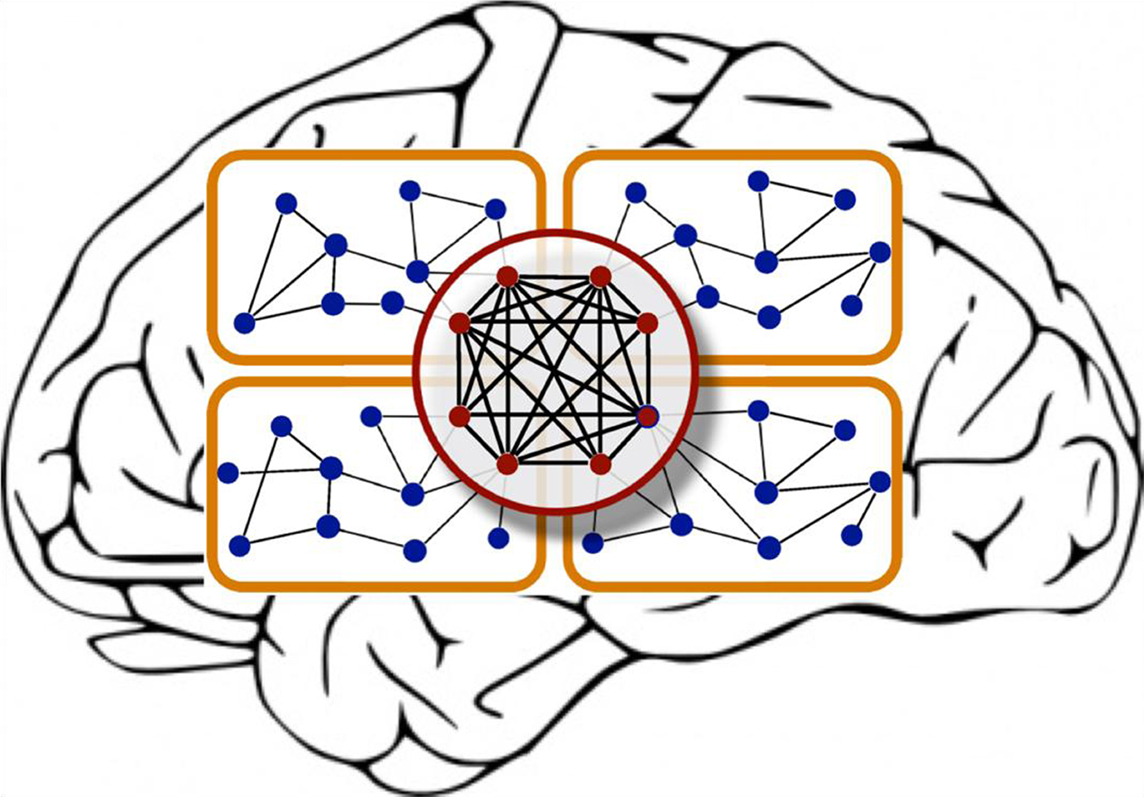
\includegraphics[height=2.5cm]{images/neuralnetwork.jpg}};
\end{tikzpicture}
\begin{itemize}
\pause
  \item Είναι ένα σύστημα επεξεργασίας πληροφοριών.\pause
  \item Τα στοιχεία που αποτελούν ένα νευρωνικό δίκτυο ονομάζονται νευρώνες.\pause
  \item Κάθε νευρώνας είναι συνδεδεμένος με άλλους νευρώνες μέσω  καθοδηγούμενων  συνδέσεων.\pause
  \item  Η κάθε σύνδεση έχει το δικό της σχετικό βάρος.
\end{itemize}
\end{frame}

%------------------------------------------------

\subsection{Πλεονεκτήματα}

\begin{frame}
\frametitle{Πλεονεκτήματα χρήσης ν.δ.}
\begin{tikzpicture}[remember picture,overlay]
\node[anchor=north east,yshift=-140pt] at (current page.north east) {
\includegraphics[height=3cm]{images/nn2.jpg}};
\end{tikzpicture}
\begin{itemize}
\pause
  \item Παράλληλα κατανεμημένη δομή\pause
  \item Ικανότητα γενίκευσης\pause
  \item Προσαρμοστικότητα\pause
  \item Ανοχή στα σφάλματα\pause
  \item Αντιστοίχηση εισόδων/εξόδων\pause
  \item Άμεση απόκριση
\end{itemize}
\end{frame}

%------------------------------------------------

\section{Ασαφή Συστήματα}

\subsection{Ασαφή Σύνολα}

\begin{frame}
\frametitle{Ασαφή Σύνολα}
\begin{itemize}
  \item Επινοήθηκαν το 1965 από τον Lotfi Zadeh\pause
  \item Μια μεταβλητή μπορεί να ανήκει μερικώς σε ένα ή περισσότερα σύνολα
    \note[item]<2>{Παράδειγμα ύψους}
\end{itemize}
\centering
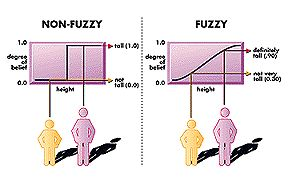
\includegraphics[height=2cm]{images/fuzzy.jpg}
\end{frame}

%\subsection{Αποσαφοποίηση}
%
%\begin{frame}
%\frametitle{Αποσαφοποίηση}
%Τι είναι;
%\end{frame}

\subsection{Συναρτήσεις Συμμετοχής}

\begin{frame}[t]
\frametitle{Συναρτήσεις Συμμετοχής}
\begin{itemize}
  \item Ορίζουν το πόσο πολύ μια μεταβλητή ανήκει σε ένα σύνολο\pause
  \item Σύνολο τιμών: $[0, 1]$\pause
\end{itemize}
\begin{center}
    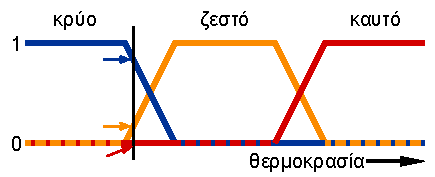
\includegraphics[height=2.5cm]{images/temperatureMF.pdf}
    \note<3>{Μια μεταβλητή μπορεί να ανήκει σε πολλά σύνολα}
\end{center}
\end{frame}

\begin{frame}[t]
\centering
\vspace{-7pt} %hack hack hack!
\frametitle{Παραδείγματα Σ.Σ.}
\begin{scriptsize}
    \begin{tabular}{@{}llc@{}}
        \toprule
        Ονομασία    & Τύπος           & Γράφημα   \\ \midrule
        Τριγωνική   & \tiny\trigLabel & \trigPlot \\
        Τραπεζοειδή & \tiny\trapLabel & \trapPlot \\
        Γκαουσιανή  & \tiny\gausLabel & \gausPlot \\ \bottomrule
    \end{tabular}
\end{scriptsize}
\end{frame}

\subsection{Φράκτες}

\begin{frame}
\frametitle{Φράκτες}
Οι φράκτες είναι τροποποιητές που εφαρμόζονται στις συναρτήσεις συμμετοχής και βοηθούν να οριστούν φράσεις όπως «λίγο», «πολύ», κτλ\pause
\begin{table}[h]
\begin{tabular}{@{}ccc@{}}
\toprule
Λίγο ($f^{1.3}\left(x\right)$) & Πολύ ($f^2\left(x\right)$) & Περίπου ($\sqrt{f\left(x\right)}$) \\ \midrule

\begin{tikzpicture}
  \begin{axis}[scale = 0.3, axis lines=none]
    \addplot[domain=0:4, blue, samples=100, ultra thick] {(trig(x))};
    \addplot[domain=0:4, red, samples=100, ultra thick] {(trig(x))^1.3};
  \end{axis}
\end{tikzpicture}

&

\begin{tikzpicture}
  \begin{axis}[scale = 0.3, axis lines=none]
    \addplot[domain=0:4, blue, samples=100, ultra thick] {(trig(x))};
    \addplot[domain=0:4, red, samples=100, ultra thick] {(trig(x))^2};
  \end{axis}
\end{tikzpicture}

&

\begin{tikzpicture}
  \begin{axis}[scale = 0.3, axis lines=none]
    \addplot[domain=0:4, blue, samples=100, ultra thick] {(trig(x))};
    \addplot[domain=0:4, red, samples=100, ultra thick] {sqrt(trig(x))};
  \end{axis}
\end{tikzpicture}

\\ \bottomrule
\end{tabular}
\end{table}
\end{frame}

\subsection{Πράξεις Συνόλων}

\begin{frame}
\frametitle{Πράξεις Συνόλων}
Έστω οι συναρτήσεις συμμετοχής $\mu_A$ και $\mu_B$ που ορίζουν τα ασαφή σύνολα $A$ και $B$ αντίστοιχα. Οι πράξεις μεταξύ των συνόλων ορίζονται ως εξής:
\begin{table}[h]
\begin{small}
\begin{tabular}{@{}ll@{}}
    \toprule
    Πράξη             & Τύπος\\ \midrule
    Ένωση (OR)        & $\mu_{A \cup B}\left(x\right) = \max\left(\mu_{A}\left(x\right), \mu_{B}\left(x\right)\right)$ \\
    Τομή (AND)        & $\mu_{A \cap B}\left(x\right) = \min\left(\mu_{A}\left(x\right), \mu_{B}\left(x\right)\right)$ \\
    Συμπλήρωμα (NOT)  & $\mu'_{A}\left(x\right) = 1 - \mu_{A}\left(x\right)$ \\ \bottomrule
\end{tabular}
\end{small}
\end{table}
\end{frame}

%------------------------------------------------

\section{Ασαφή Συστήματα Συμπερασμού}

\begin{frame}
\frametitle{Ασαφή Συστήματα Συμπερασμού}
\begin{itemize}
  \item Συστήματα που αντιστοιχίζουν τιμές από έναν χώρο εισόδου σε έναν χώρο εξόδου\pause
  \item Γίνεται με την χρήση ΕΑΝ-ΤΟΤΕ κανόνων\pause
  \item \textit{Εάν η ταχύτητα είναι \textbf{μικρή} και η επιτάχυνση \textbf{μικραίνει}, τότε πάτα \textbf{λίγο} γκάζι}
\end{itemize}
\end{frame}

\subsection{Δομή ενός ασαφούς συστήματος}

\begin{frame}
\frametitle{Δομή ενός ασαφούς συστήματος}
\centering
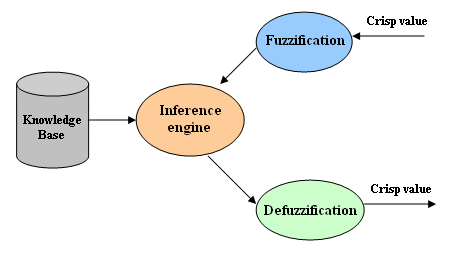
\includegraphics[height=5cm]{images/modulosfis_en.png}
\end{frame}

\subsection{Mamdani}

\begin{frame}
\frametitle{Γενικά για το Α.Σ.Σ. Mamdani}
\begin{itemize}
  \item Είναι από τις πιο διαδεδομένες μεθοδολογίες στον χώρο των Α.Σ.\pause
  \item Ήταν από τα πρώτα συστήματα ελέγχου που χρησιμοποίησαν θεωρία ασαφών συνόλων\pause
  \item Προτάθηκε το 1975 από τον Ebrahim Mamdani για τον έλεγχο ενός συνδυασμού ατμομηχανής με βραστήρα.
\end{itemize}
\end{frame}

\begin{frame}
\frametitle{Βήματα δημιουργίας και υπολογισμού}
\begin{enumerate}
  \item Δημιουργία ασαφών κανόνων\pause
  \item Ασαφοποίηση\pause
  \item Ασαφείς συνδυασμοί\pause
  \item Εξαγωγή αποτελέσματος\pause
  \item Συνδυασμός των αποτελεσμάτων\pause
  \item Αποσαφοποίηση
\end{enumerate}
\end{frame}

\begin{frame}
\frametitle{Παράδειγμα}
\centering
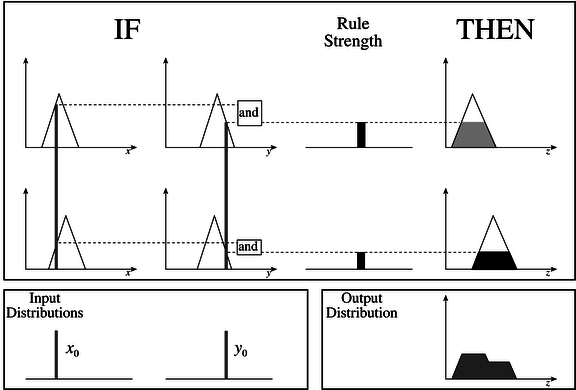
\includegraphics[height=5cm]{images/fuzzy001.png}
\end{frame}

\subsection{Sugeno}

\begin{frame}
\frametitle{Γενικά για το Α.Σ.Σ. Sugeno}
\begin{itemize}
  \item Γνωστό κι ως TSK (από τα αρχικά των κατασκευαστών Takagi-Sugeno-Kang)\pause
  \item Παρόμοιο με το Mamdani, αλλά δεν υπάρχει συνάρτηση συμμετοχής για την έξοδο\pause
  \item Εάν Είσοδος $1 = x$ και Είσοδος $2 = y$ τότε Έξοδος $z = ax + by + c$\pause
  \item Υπάρχουν αλγόριθμοι για την βελτιστοποίηση του FIS (adaptive neuro-fuzzy inference system \textendash ANFIS)
\end{itemize}
\end{frame}

%------------------------------------------------

\section{Συσταδοποίηση και Ομαδοποίηση}

\subsection{Ορισμός Συσταδοποίησης}

\begin{frame}
\frametitle{Ορισμός Συσταδοποίησης}
\begin{itemize}
  \item Διαδικασία ομαδοποίησης αντικειμένων με κάποιο κοινό χαρακτηριστικό.\pause
  \item Χαρακτηρίζεται και ως μάθηση χωρίς επίβλεψη.
\end{itemize}
\end{frame}

\subsection{Στάδια Συσταδοποίησης}

\begin{frame}
\frametitle{Στάδια Συσταδοποίησης}
\begin{itemize}
  \item Αναπαράσταση των προτύπων και εξαγωγή των χαρακτηριστικών τους.\pause
  \item Επιλογή  του  κατάλληλου  αλγορίθμου.\pause
  \item Ομαδοποίηση των δεδομένων και αξιολόγηση των αποτελεσμάτων του αλγορίθμου.\pause
  \item Αξιολόγηση του τελικού αποτελέσματος και ερμηνεία των αποτελεσμάτων.
\end{itemize}
\end{frame}

\subsection{Αλγόριθμοι Συσταδοποίησης}

\begin{frame}
\frametitle{Αλγόριθμοι}
\begin{itemize}
  \item Ιεραρχική Συσταδοποίηση\pause
  \item Διαμεριστική Συσταδοποίηση\pause
  \item Ασαφής Συσταδοποίηση
\end{itemize}
\end{frame}

%------------------------------------------------

\begin{frame}
\frametitle{Ορισμός Ομαδοποίησης}
\begin{itemize}
  \item Διαδικασία ενσωμάτωσης ενός νέου αντικειμένου σε μια ομάδα με τη βοήθεια της εκπαίδευσης.\pause
  \item Προκύπτει από μια σειρά δεδομένων των οποίων ο διαχωρισμός είναι γνωστός αναφέρεται και ως αναγνώριση  προτύπων ή μάθηση υπό επίβλεψη.
\end{itemize}
\end{frame}

%------------------------------------------------

\section{Παρουσίαση και επίλυση του προβλήματος}
\subsection{Παρουσίαση του προβλήματος}
\begin{frame}
\frametitle{Παρουσίαση του προβλήματος}
\begin{itemize}
  \item Δημιουργία ενός ασαφούς μοντέλου τύπου TSK για την ταξινόμηση κρίνων σε 3 κατηγορίες (setosa, versicolor και virginica).\pause
  \item Χρήση μιας συλλογής 150 δειγμάτων.\pause
  \item Τα 75 δείγματα θα χρησιμοποιηθούν για την εκπαίδευση και τα υπόλοιπα 75 για τον έλεγχο της ικανότητας ταξινόμησης του.
\end{itemize}
\end{frame}

%------------------------------------------------

\subsection{Φόρτωμα Δεδομένων}

\begin{frame}[fragile]
\frametitle{Φόρτωμα Δεδομένων}
Συνάρτηση που επιστρέφει σε μεταβλητές τα δεδομένα των κρίνων
\begin{lstlisting}
function [iris, shuffledIris, irisTrain, irisTest, irisTrainIn, ...
    irisTrainOut, irisTestIn, irisTestOut] = getIris(trainingSize)

    load iris.dat;

    shuffledIris = iris(randperm(size(iris, 1)), :);
    irisTrain = shuffledIris(1:trainingSize, :);
    irisTest = shuffledIris((trainingSize + 1):150, :);

    irisTrainIn = irisTrain(:, 1:4);
    irisTrainOut = irisTrain(:, 5);
    irisTestIn = irisTest(:, 1:4);
    irisTestOut = irisTest(:, 5);
end
\end{lstlisting}
\end{frame}

\subsection{Επίλυση με χρήση γραφικού περιβάλλοντος}

\subsubsection{Fuzzy Toolbox}
\begin{frame}
\frametitle{Fuzzy Toolbox}
\centering
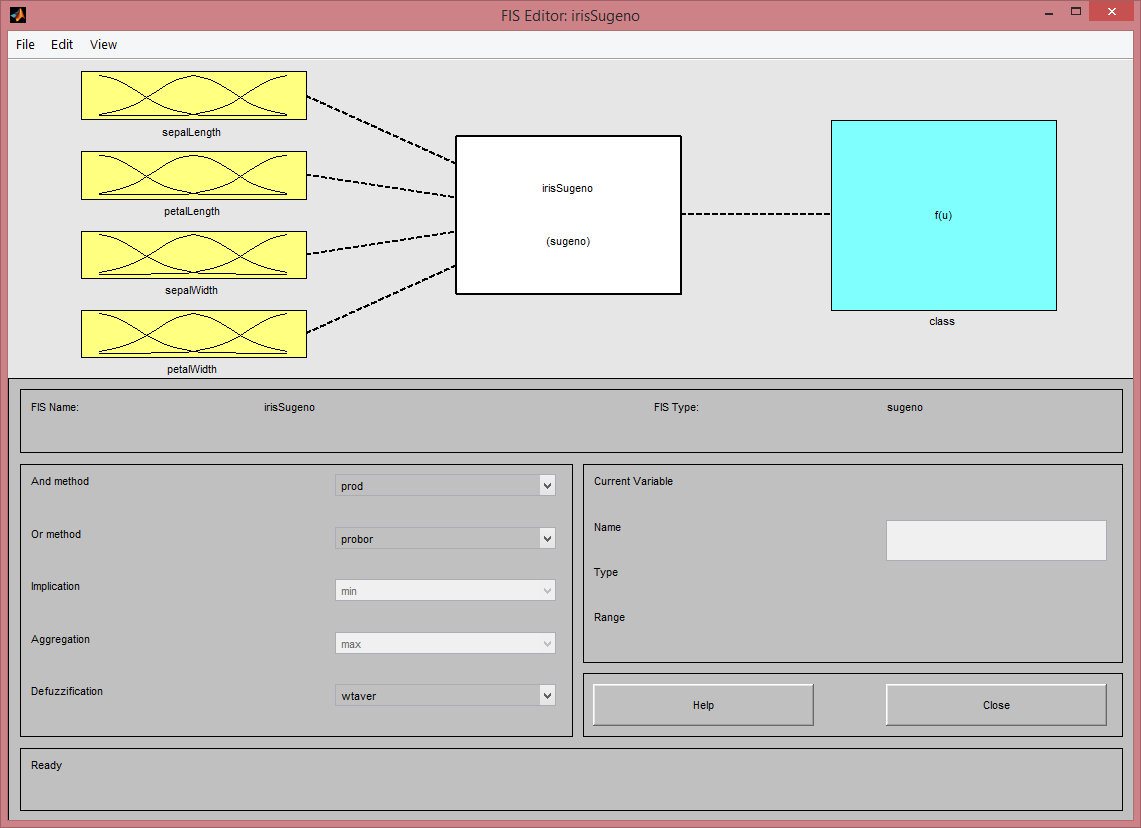
\includegraphics[height=5.5cm]{images/fuzzySugeno.png}
\end{frame}

\subsubsection{Anfis Editor}
\begin{frame}
\frametitle{Anfis Editor}
\centering
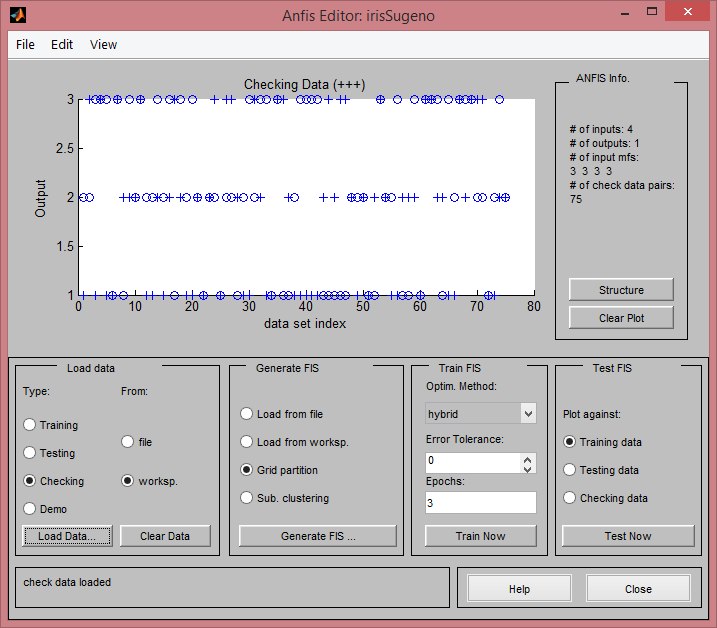
\includegraphics[height=5.5cm]{images/ANFIS.png}
\end{frame}

\subsubsection{Grid Partition}
\begin{frame}
\frametitle{Grid Partition}
\centering
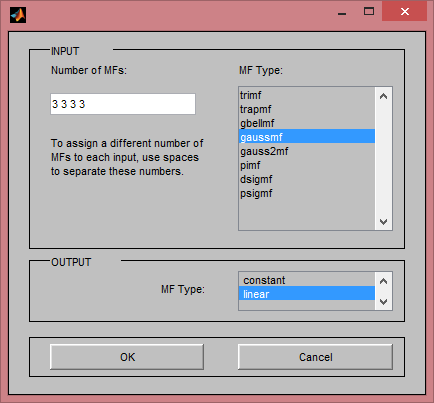
\includegraphics[height=4.5cm]{images/gridParam.png}
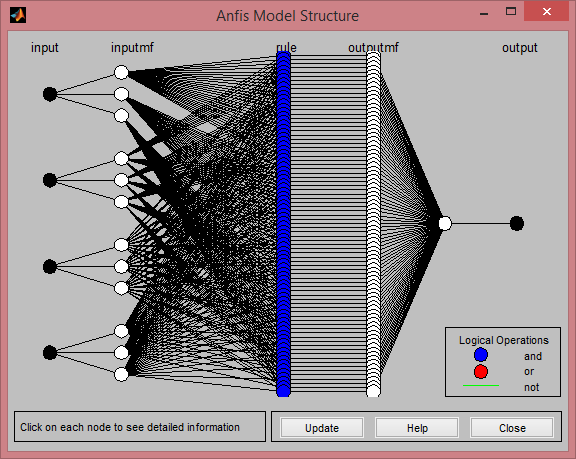
\includegraphics[height=4.5cm]{images/anfisModelGrid.png}

\end{frame}

\subsubsection{Subtractive Clustering}
\begin{frame}
\frametitle{Subtractive Clustering}
\centering
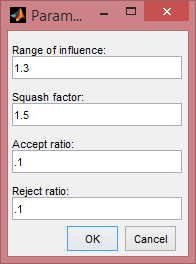
\includegraphics[height=4.5cm]{images/subParam.png}
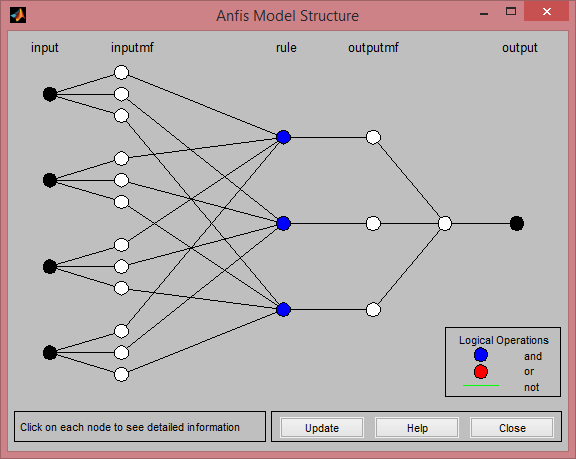
\includegraphics[height=4.5cm]{images/anfisModelSub.png}
\end{frame}

\subsubsection{Αποτελέσματα}
\begin{frame}
\frametitle{Αποτελέσματα}
\centering
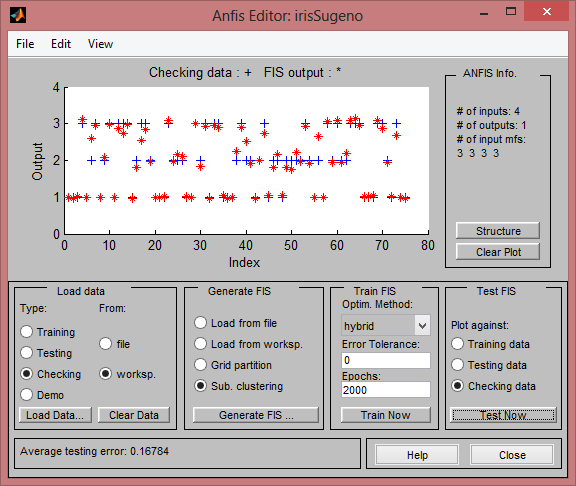
\includegraphics[height=5.5cm]{images/ANFIS_results.png}
\end{frame}

\subsection{Επίλυση με χρήση κώδικα}
\begin{frame}
\frametitle{Ανάγκη χρήσης κώδικα}
\begin{itemize}
  \item Μεγάλο μέσο τετραγωνικό σφάλμα\pause
  \item Επιστρέφει πραγματικές τιμές και όχι ακέραιες\pause
  \item Λύση: Στρογγυλοποίηση των τιμών
\end{itemize}
\end{frame}

%\subsubsection{setSeed.m}
%\begin{frame}
%\frametitle{setSeed.m}
%Τι είναι;
%\end{frame}

\subsubsection{irisClustering.m}
\begin{frame}[fragile]
\frametitle{irisClustering.m}
\small{Συνάρτηση που κάνει την κατηγοριοποίηση και επιστρέφει πόσα λάθη έγιναν}
\begin{lstlisting}
function [badTrainFis, badCheckFis] = irisClustering ...
    (seed, radius, squashFactor, acceptRatio, rejectRatio, epochs)

    fis = genfis2(irisTrainIn, irisTrainOut, radius, ...
        [min(iris); max(iris)], [squashFactor acceptRatio rejectRatio 0]);

    [trainFis, trainError, stepSize, checkFis, checkError] = ...
        anfis(irisTrain, fis, epochs, [], irisTest);

    trainFisOut = round(evalfis(irisTestIn, trainFis));
    badTrainFis = size(find((trainFisOut == irisTestOut) == 0), 1);

    checkFisOut = round(evalfis(irisTestIn, checkFis));
    badCheckFis = size(find((checkFisOut == irisTestOut) == 0), 1);
end
\end{lstlisting}
\end{frame}

\subsubsection{runTests.m}
\begin{frame}[fragile]
\frametitle{runTests.m}
Εκτελεί την κατηγοριοποίηση με διαφορές παραμέτρους
\begin{lstlisting}
for radius = 0.6:0.1:1.5
    for squashFactor = 0.5:0.5:4
        for acceptRatio = 0.1:0.5:2
            for rejectRatio = 0.1:0.5:2
                [badTrainFis, badCheckFis] = ...
                    irisClustering(0, radius, squashFactor, ...
                    acceptRatio, rejectRatio, 2000);
                runs = [runs; radius squashFactor acceptRatio ...
                    rejectRatio badTrainFis badCheckFis];
            end
        end
    end
end
\end{lstlisting}
\end{frame}

\subsection{Αποτελέσματα}
\begin{frame}
\frametitle{Αποτελέσματα}
Καλύτερα αποτελέσματα: Subtractive clustering

\begin{table}
    \centering
    \begin{small}
        \begin{tabular}{@{}lr@{}}
            \toprule
            Παράμετρος    & \multicolumn{1}{l}{Τιμή} \\ \midrule
            Radius        & 1.3                      \\
            Squash factor & 1.5                      \\
            Accept ratio  & 0.1                      \\
            Reject ratio  & 0.1                      \\
            Εποχές        & 2000                     \\ \bottomrule
        \end{tabular}
    \end{small}
\end{table}

Μέσος όρος λάθος ταξινομήσεων: $2.5743$
\end{frame}

%----------------------------------------------------------------------------------------


\begin{frame}

\Huge{\centerline{Thank You}}
\Large{\centerline{Questions?}}
\end{frame}

\end{document} 